% !TEX root = main.tex

\section{A brief history of bioinformatics lecture}


\paragraph{Some cool stuff}

\begin{itemize}
    \item Hemoglobin, helps showing a degree of similarity
    over long evolutionary time using the gen variations.
    \item Pairwise protein sequence alignments: \\
    (dot-matrix methods, dynamic programming and word methods)
    \item Needleman–Wunsch algorithm. \\
    (computationally impractical)
    \[O(L^{N})\]
    Where L is sequence length and N the amount of sequences
\end{itemize}
\paragraph{\\}
\begin{figure}[htbp]
    \centerline{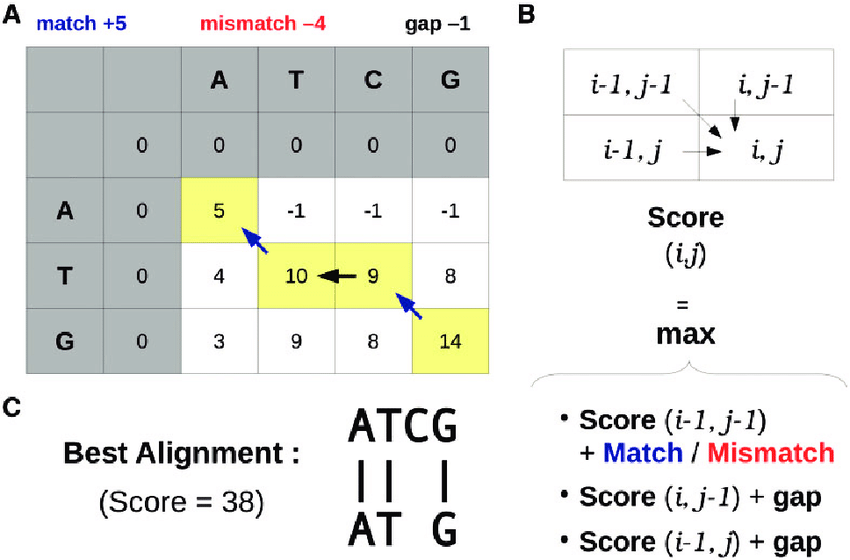
\includegraphics[width=200mm]{Needleman.png}}
    \caption{Needleman–Wunsch algorithm}
    \label{fig5}
\end{figure}

\paragraph*{Progressive sequence alignment} 

\begin{itemize}
    \item Performing a Needleman–Wunsch alignment for all sequence pairs.
    \item Extracting pairwise similarity scores for eachpairwise alignment.
    \item Using those scores to build a guide tree and then... 
    \item Aligning the two most similar sequences, and then
    the next more similar sequence, and so on, according to the
    guide tree.
\end{itemize}

\paragraph*{CLUSTAL software (Feng–Doolittle algorithm)} 

\paragraph*{Maxam–Gilbert sequencing method 1976} 




